\documentclass{article}

\PassOptionsToPackage{numbers,sort&compress}{natbib}
\usepackage[preprint]{neurips_2021}
\usepackage[utf8]{inputenc}
\usepackage[T1]{fontenc}
\usepackage{hyperref}
\usepackage{url}
\usepackage{booktabs}
\usepackage{amsfonts}
\usepackage{nicefrac}
\usepackage{microtype}
\usepackage{xcolor}
\usepackage{graphicx}
\usepackage{subcaption}
\usepackage{multirow}
\usepackage{array}
\usepackage{float}
\usepackage{adjustbox}
\usepackage{amsthm}
\usepackage{amsmath}
\usepackage{amssymb}
\usepackage{mathtools}
\usepackage{enumitem}
\usepackage{algorithm}
\usepackage{algpseudocode}

\title{CORA: Domain Generalization by Matching the Consensus Core of the Connected Trajectory Rashomon Set}

\author{Anonymous Authors}

\newtheorem{theorem}{Theorem}
\newtheorem{proposition}{Proposition}
\newtheorem{lemma}{Lemma}
\newtheorem{corollary}{Corollary}
\newtheorem{definition}{Definition}
\newtheorem{assumption}{Assumption}
\newtheorem{remark}{Remark}

\newcommand{\RR}{\mathbb{R}}
\newcommand{\EE}{\mathbb{E}}
\newcommand{\cC}{\mathcal{C}}
\newcommand{\cU}{\mathcal{U}}
\newcommand{\cV}{\mathcal{V}}
\newcommand{\cA}{\mathcal{A}}
\newcommand{\cI}{\mathcal{I}}
\newcommand{\argmin}{\operatorname*{arg\,min}}
\newcommand{\argmax}{\operatorname*{arg\,max}}
\newcommand{\KL}{\operatorname{KL}}
\newcommand{\TV}{\operatorname{TV}}
\newcommand{\diam}{\operatorname{diam}}
\newcommand{\TBD}{\textbf{TBD}}
\newcommand{\etal}{\textit{et al.}}
\newcommand{\ie}{\textit{i.e.}}
\newcommand{\eg}{\textit{e.g.}}
\newcommand{\iid}{i.i.d.}
\newcommand{\ood}{OOD}
\newcommand{\iidcaps}{IID}
\newcommand{\cora}{\textup{\textsc{CORA}}}
\newcommand{\swad}{\textup{\textsc{SWAD}}}
\newcommand{\stawa}{\textup{\textsc{STAWA}}}
\newcommand{\dcola}{\textup{\textsc{D-COLA}}}
\newcommand{\diwa}{\textup{\textsc{DiWA}}}
\newcommand{\miro}{\textup{\textsc{MIRO}}}
\newcommand{\norm}[1]{\left\lVert #1 \right\rVert}
\newcommand{\inner}[2]{\left\langle #1, #2 \right\rangle}
\newcommand{\simplex}{\Delta}

\begin{document}

\maketitle

\begin{abstract}
Single-run post-hoc methods matter in domain generalization because they can be attached to strong empirical risk minimization pipelines without retraining. The canonical method in this regime is \swad, which selects and averages dense checkpoints by seeking flat minima in parameter space. Subsequent work such as \diwa{} and adjacent literature on predictive multiplicity suggest that flatness is only part of the story: good post-hoc solutions can require nonuniform soups of complementary checkpoints, while checkpoint-level calmness alone can collapse back to ordinary validation selection. We propose \textbf{Consensus-of-Rashomon Averaging} (\cora), a new label-free single-run post-hoc DG method that changes the object of optimization from flatness or global drift to the \emph{predictive consensus core} of the connected set of near-optimal checkpoints. Starting from one dense trajectory, \cora{} first constructs a connected trajectory Rashomon set using pooled validation loss and a soup-safety barrier, then forms the predictive barycenter of that set on a held-out support pool, computes an examplewise multiplicity score, and finally solves a convex simplex optimization that matches the barycenter on low-multiplicity examples while hedging against arbitrary labels on the high-multiplicity fringe. We prove that the barycenter is the information projection of the candidate set, that the \cora{} objective is convex, that its support-side core/fringe term yields a target-risk certificate under an explicit consensus-fringe decomposition, that the empirical objective concentrates uniformly over the simplex, that the optimized predictive mixture transfers to a single weight soup under a local second-order linearity condition, and that \cora{} optimizes over a strictly richer feasible family than any \swad-style contiguous uniform interval once the same certificate is accepted. We also prove a concrete separation result showing that validation-equivalent soups can still differ in fringe ambiguity in a way that \cora{} detects and validation-only selection misses. New \cora{} empirical results are intentionally left as \TBD{} pending execution; however, we include exact published baseline numbers from \swad, \diwa, and \miro{} to define the current frontier.
\end{abstract}

\section{Introduction}

Domain generalization (DG) asks for a model that performs well on an unseen target environment using only source data at training time. In practice, the methods that have mattered most are often the ones that keep the underlying training pipeline intact and change only the post-hoc model-selection rule. \swad{} \citep{cha2021swad} is the canonical example: on the standard DomainBed ResNet-50 protocol it improves ERM from `63.3' to `66.9' average \ood{} accuracy across PACS, VLCS, OfficeHome, TerraIncognita, and DomainNet \citep{cha2021swad}. Its appeal is broader than one benchmark table. It is single-run, one-model at test time, and easy to integrate.

Yet the surrounding literature points to a deeper story. \diwa{} \citep{rame2022diwa} argues that weight averaging helps not only because of flatness, but because of diversity, covariance, and locality; in its strongest LP multi-run setting it reaches `68.0' average accuracy on the five-dataset benchmark family \citep{rame2022diwa}. \miro{} \citep{cha2022miro} shows that preserving transferable structure from pretraining is largely orthogonal to post-hoc averaging, reaching `65.9' on its own and `68.1' when combined with \swad{} \citep{cha2022miro}. These are not directly identical protocols, but together they suggest that the next post-hoc DG method should not merely optimize \emph{which checkpoint} or \emph{which contiguous window} to trust. It should optimize \emph{what the near-optimal checkpoints actually agree on}.

This paper proposes that object. Our starting point is the connected \emph{trajectory Rashomon set}: the set of checkpoints from one dense run that are both near-optimal in pooled source validation loss and safely averageable by a connectivity test. The key observation is that near-optimal checkpoints can still disagree on individual examples. Some examples are predicted almost identically by the whole set; others sit in a disagreement fringe. We call the former the \emph{consensus core} and the latter the \emph{high-multiplicity fringe}. Our central claim is:
\begin{quote}
Among single-run post-hoc soups that are safe to average, the best DG candidate is the one that matches the predictive barycenter on the consensus core and hedges on the high-multiplicity fringe.
\end{quote}

This leads to \cora{}: \textbf{C}onsensus-\textbf{o}f-\textbf{R}ashomon \textbf{A}veraging. For each support example, \cora{} computes the predictive barycenter of the candidate checkpoint set, an examplewise predictive multiplicity score, and a core weight. It then solves a convex simplex optimization with three terms: pooled source validation fit, barycenter-matching on low-multiplicity examples, and a worst-case ambiguity penalty on high-multiplicity examples. The output is still a single test-time model obtained by weight averaging.

Why is this different from existing methods?
\begin{itemize}[leftmargin=1.4em]
    \item \swad{} searches for a wide contiguous basin in parameter space.
    \item \stawa{} searches for a functionally calm checkpoint or plateau over time.
    \item \dcola{} searches for a safe, diverse checkpoint soup using checkpoint-level global statistics.
    \item \cora{} searches for the soup that best matches the \emph{predictive center of the connected good-model set itself}.
\end{itemize}

This is the conceptual shift. The new object is not weight-space flatness, not global trajectory calmness, and not checkpoint-level covariance alone. It is \emph{predictive multiplicity structure}.

The paper's main contributions are:
\begin{enumerate}[leftmargin=1.4em]
    \item We introduce \cora{}, a label-free, single-run post-hoc DG method built around the connected trajectory Rashomon set, its predictive barycenter, and an examplewise multiplicity decomposition into a consensus core and a high-multiplicity fringe.
    \item We prove that the barycenter is the unique information projection of the candidate set, and that the \cora{} objective is convex with a unique minimizer when the simplex entropy term is active.
    \item We derive a target-risk certificate under an explicit consensus-fringe decomposition: the core term appears as a KL transfer term to the barycenter, and the fringe term appears as a worst-case log-loss ambiguity term.
    \item We prove uniform concentration of the support-side objective over the simplex, projected-subgradient convergence for the post-hoc optimizer, and a predictive-mixture to single-weight-soup transfer bound under a local second-order linearity condition.
    \item We prove a conditional domination result: under the same certificate, \cora{} achieves a no-worse certificate than any feasible \swad-style uniform interval, and we provide a constructive separation example where validation-equivalent soups can still have sharply different fringe ambiguity and target risk.
    \item We provide a full NeurIPS-style manuscript with proofs, algorithm box, analytical visuals, exact published baselines from prior work, and a \TBD{}-only section for all new \cora{} experiments.
\end{enumerate}

\begin{remark}
We do \emph{not} claim an unconditional theorem that \cora{} empirically dominates \swad{}, \diwa{}, \dcola{}, or every other DG method on every benchmark. That would be indefensible. The strongest honest statement is that \cora{} optimizes a different object, that this object yields a stronger certificate under explicit assumptions, and that validation-only or interval-only selectors provably miss it on a nontrivial class of examples.
\end{remark}

\begin{figure}[t]
    \centering
    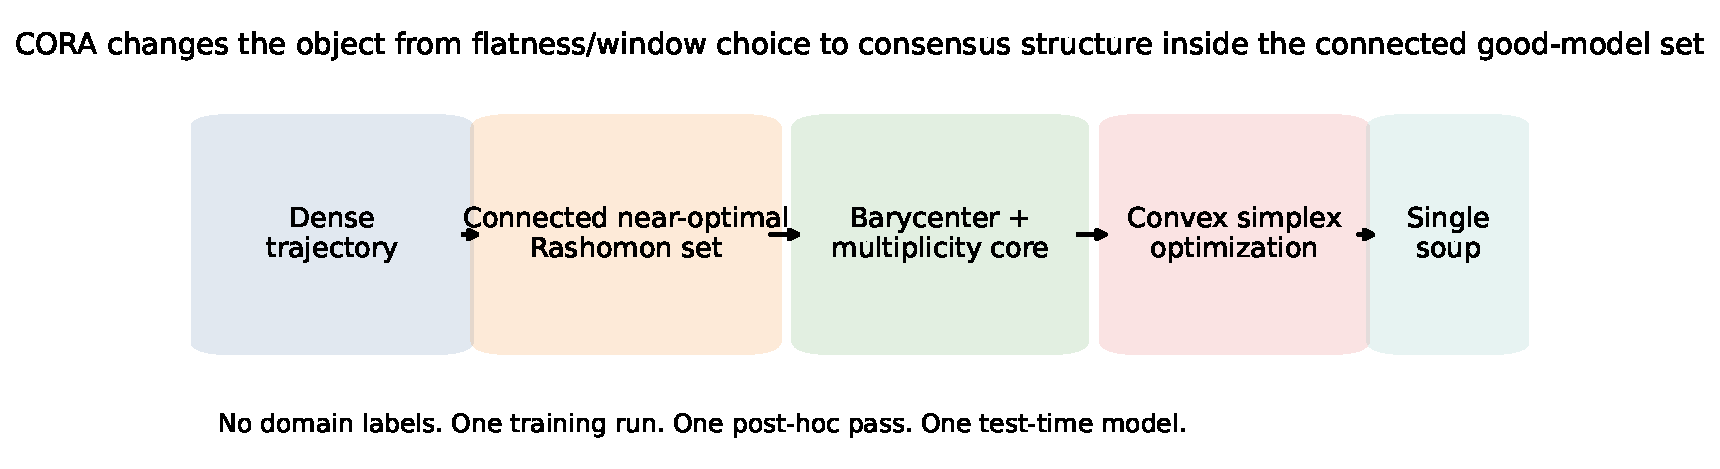
\includegraphics[width=\linewidth]{figures/cora_overview.pdf}
    \caption{\textbf{\cora{} overview.} Starting from one dense trajectory, \cora{} constructs a connected near-optimal checkpoint set, computes a predictive barycenter over that set, estimates examplewise multiplicity to define a consensus core and disagreement fringe, and solves a convex post-hoc simplex problem whose output is a single weight soup.}
    \label{fig:overview}
\end{figure}

\section{Related Work}

\paragraph{Single-run post-hoc DG.}
\swad{} \citep{cha2021swad} is the canonical single-run post-hoc DG method. Its practical appeal comes from dense checkpoint sampling, overfit-aware window selection, and a final weight average. Stationarity-style selectors attempt to move the object from weight-space geometry to function-space dynamics, but checkpoint-level calmness alone need not identify the best soupable subset of a trajectory. \cora{} stays in the single-run regime while changing the object from checkpoint scoring to structure inside the connected set of good checkpoints.

\paragraph{Weight averaging, connectivity, and soups.}
SWA \citep{izmailov2018swa}, mode connectivity \citep{garipov2018fge}, and model soups \citep{wortsman2022soups} established that averaging nearby models can improve generalization when they lie in a connected low-loss region. \diwa{} \citep{rame2022diwa} sharpened this story for \ood{} settings by emphasizing diversity, covariance, and locality. \cora{} inherits the connectivity constraint and the nonuniform soup scaffold, but changes the target from checkpoint-level redundancy to example-level consensus structure.

\paragraph{Predictive multiplicity and churn.}
The Rashomon-set literature argues that many near-optimal models can coexist and disagree materially on individual predictions \citep{hsu2022rashomon,watsondaniels2024churn}. Predictive churn work treats such disagreement across updates or model sets as a first-class deployment concern rather than harmless noise \citep{watsondaniels2024churn}. \cora{} imports this perspective into post-hoc DG: a checkpoint set should not only be low-loss and averageable, but should also reveal which examples are truly agreed upon.

\paragraph{Stability and non-convergent training.}
Algorithmic stability is one route to generalization \citep{bousquet2002stability,hardt2016sgd}. More recently, \citet{chandramoorthy2022nonconvergent} showed that stable long-run dynamics, not literal fixed-point convergence, are the relevant object for learning algorithms that do not converge. \cora{} is consistent with this perspective, but instead of checkpoint-level drift it uses the completed trajectory to estimate a stable predictive core.

\paragraph{Pretraining-aware DG.}
\miro{} \citep{cha2022miro} shows that preserving information from a broader pretraining prior is largely orthogonal to post-hoc averaging. This supports a useful design principle for \cora{}: source fit should remain explicit, while the support-side regularizer should measure a distinct transfer-relevant object rather than rediscovering validation loss.

\section{Problem Setup}
\label{sec:setup}

We focus on multiclass classification, the standard regime of the DomainBed benchmarks. Let a single training run produce dense checkpoints $\{\theta_t\}_{t=1}^{K}$. We reserve:
\begin{itemize}[leftmargin=1.4em]
    \item a pooled labeled source-validation set $\cV = \{(x_j,y_j)\}_{j=1}^{n}$ used for post-hoc checkpoint scoring and barrier tests, and
    \item a pooled unlabeled support set $\cU = \{x_i\}_{i=1}^{m}$ used to estimate predictive multiplicity.
\end{itemize}
Neither set requires domain labels.

For classification, let
\[
    p_t(x) \in \simplex^{K_{\mathrm{cls}}-1}
\]
denote the class-probability vector predicted by checkpoint $\theta_t$ at input $x$. We define the pooled validation loss
\begin{equation}
    L_{\cV}(\theta_t)
    \triangleq
    \frac{1}{n}\sum_{j=1}^{n} -\log p_t(x_j)_{y_j}.
    \label{eq:val_loss}
\end{equation}

To guarantee that soups remain inside one connected low-loss region, we use a pooled interpolation barrier to an anchor checkpoint $a$:
\begin{equation}
    B(t,a)
    \triangleq
    \max_{\alpha \in \cA}
    L_{\cV}\!\big((1-\alpha)\theta_a + \alpha \theta_t\big)
    -
    \max\{L_{\cV}(\theta_a), L_{\cV}(\theta_t)\},
    \label{eq:barrier}
\end{equation}
where $\cA \subset [0,1]$ is a fixed interpolation grid.

The anchor is the lowest pooled-validation checkpoint:
\begin{equation}
    a \in \argmin_{1 \le t \le K} L_{\cV}(\theta_t).
    \label{eq:anchor}
\end{equation}
The connected near-optimal checkpoint set is
\begin{equation}
    \cC
    \triangleq
    \left\{
        t :
        L_{\cV}(\theta_t) \le L_{\cV}^{\star} + \epsilon,
        \;
        B(t,a) \le \tau
    \right\},
    \qquad
    L_{\cV}^{\star} = \min_t L_{\cV}(\theta_t).
    \label{eq:candidate_set}
\end{equation}
This is our \emph{connected trajectory Rashomon set}: the set of checkpoints that are simultaneously near-optimal and soup-safe.

\section{Consensus-of-Rashomon Averaging}
\label{sec:method}

\subsection{Trajectory prior and predictive barycenter}

We first define a soft prior over the connected candidate set:
\begin{equation}
    \rho_t
    \triangleq
    \frac{
        \exp\!\left(-\beta [L_{\cV}(\theta_t)-L_{\cV}^{\star}] - \nu B(t,a)\right)
    }{
        \sum_{s\in\cC}
        \exp\!\left(-\beta [L_{\cV}(\theta_s)-L_{\cV}^{\star}] - \nu B(s,a)\right)
    },
    \qquad
    t \in \cC,
    \label{eq:rho}
\end{equation}
where $\beta,\nu \ge 0$.

For each support example $x_i \in \cU$, the \emph{predictive barycenter} of the candidate set is
\begin{equation}
    q_i
    \triangleq
    \sum_{t\in\cC} \rho_t p_t(x_i).
    \label{eq:barycenter}
\end{equation}

\begin{theorem}[Barycenter optimality]
\label{thm:barycenter}
Fix any support example $x_i$. Among all predictive distributions $r$ in the closed simplex,
\begin{equation}
    q_i
    =
    \argmin_{r}
    \sum_{t\in\cC} \rho_t \KL\!\big(p_t(x_i) \,\|\, r\big).
    \label{eq:barycenter_opt}
\end{equation}
If every class receives nonzero total mass under $\{p_t(x_i)\}_{t\in\cC}$, the minimizer is unique.
\end{theorem}

This theorem justifies the object that \cora{} tries to match. It is not an arbitrary average; it is the unique information projection center of the connected good-model set for that example.

\subsection{Predictive multiplicity and the consensus core}

For each support example, define its predictive multiplicity
\begin{equation}
    M_i
    \triangleq
    \sum_{t\in\cC} \rho_t \KL\!\big(p_t(x_i)\,\|\,q_i\big).
    \label{eq:multiplicity}
\end{equation}

Low $M_i$ means that near-optimal checkpoints largely agree on $x_i$; high $M_i$ means that $x_i$ lies in the disagreement fringe. We convert multiplicity into a soft consensus-core weight
\begin{equation}
    c_i
    \triangleq
    \exp(-\kappa M_i),
    \qquad
    \kappa \ge 0.
    \label{eq:core_weight}
\end{equation}
Examples with high $c_i$ belong to the consensus core. Examples with low $c_i$ belong to the high-multiplicity fringe.

\subsection{Predictive-mixture objective}

For soup weights $w \in \simplex^{|\cC|}$, define the predictive mixture
\begin{equation}
    p_w(x)
    \triangleq
    \sum_{t\in\cC} w_t p_t(x).
    \label{eq:mixture}
\end{equation}

The validation loss of the predictive mixture is
\begin{equation}
    L_{\cV}^{\mathrm{ens}}(w)
    \triangleq
    \frac{1}{n}
    \sum_{j=1}^{n}
    -\log\!\Big(
        \sum_{t\in\cC} w_t p_t(x_j)_{y_j}
    \Big).
    \label{eq:ensval}
\end{equation}

The support-side \emph{core-matching} term is
\begin{equation}
    \Omega_{\mathrm{core}}(w)
    \triangleq
    \frac{1}{m}
    \sum_{i=1}^{m}
    c_i \KL\!\big(q_i \,\|\, p_w(x_i)\big).
    \label{eq:core_term}
\end{equation}

The support-side \emph{fringe ambiguity} term is
\begin{equation}
    \Omega_{\mathrm{amb}}(w)
    \triangleq
    \frac{1}{m}
    \sum_{i=1}^{m}
    (1-c_i)
    A\!\big(p_w(x_i)\big),
    \qquad
    A(p) \triangleq \max_{1\le y\le K_{\mathrm{cls}}} -\log p_y.
    \label{eq:amb_term}
\end{equation}
This is the exact worst-case single-label log loss on that example.

Finally, let $b_t = B(t,a)$ and define
\begin{equation}
    J(w)
    \triangleq
    L_{\cV}^{\mathrm{ens}}(w)
    + \lambda_{\mathrm{core}} \Omega_{\mathrm{core}}(w)
    + \lambda_{\mathrm{amb}} \Omega_{\mathrm{amb}}(w)
    + \lambda_{\mathrm{loc}} \sum_{t\in\cC} w_t b_t
    + \lambda_{\mathrm{ent}} \sum_{t\in\cC} w_t \log w_t,
    \label{eq:objective}
\end{equation}
with nonnegative coefficients. The post-hoc optimizer is
\begin{equation}
    w^{\star}
    \in
    \argmin_{w\in\simplex^{|\cC|}} J(w).
    \label{eq:optimizer}
\end{equation}

The final single model is the weight soup
\begin{equation}
    \bar \theta_{\cora}
    \triangleq
    \sum_{t\in\cC} w_t^{\star} \theta_t.
    \label{eq:final_soup}
\end{equation}

\paragraph{Implementation note.}
Our implementation follows Eqs.~\eqref{eq:rho}--\eqref{eq:final_soup} directly, with two numerical conventions. First, each predictive distribution is replaced by the affine clipped version
\[
    \tilde p=(1-K_{\mathrm{cls}}\eta)p+\eta \mathbf{1},
\]
which keeps the vector on the simplex while ensuring every class probability is at least $\eta$. Second, we optimize Eq.~\eqref{eq:optimizer} by projected gradient descent on the simplex, initialized at the trajectory prior $\rho$, and deploy the best iterate encountered. These are numerical choices for solving the stated convex program; they do not change the target objective.

\paragraph{What is genuinely new here.}
\cora{} is not just another souping rule. The new object is the pair
\[
    (q_i, c_i)
\]
over support examples:
\begin{itemize}[leftmargin=1.4em]
    \item $q_i$ is the predictive center of the connected good-model set;
    \item $c_i$ identifies whether that example lives in the consensus core or the disagreement fringe.
\end{itemize}
The optimizer matches the first and hedges on the second.

\begin{figure}[t]
    \centering
    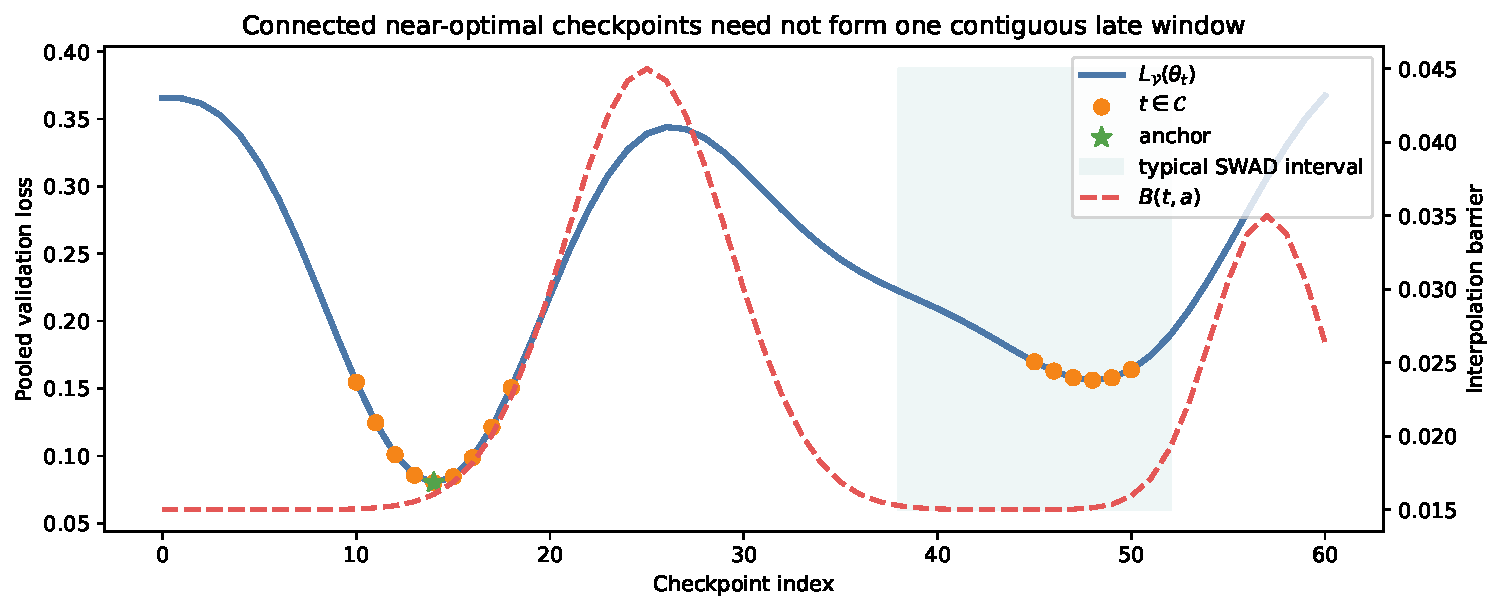
\includegraphics[width=\linewidth]{figures/connected_rashomon_set.pdf}
    \caption{\textbf{The connected near-optimal set is not necessarily a contiguous window.} \cora{} keeps the \swad{} intuition that safe soups live inside one connected region, but it replaces contiguous time windows with an explicit loss-plus-barrier feasibility test.}
    \label{fig:set}
\end{figure}

\begin{figure}[t]
    \centering
    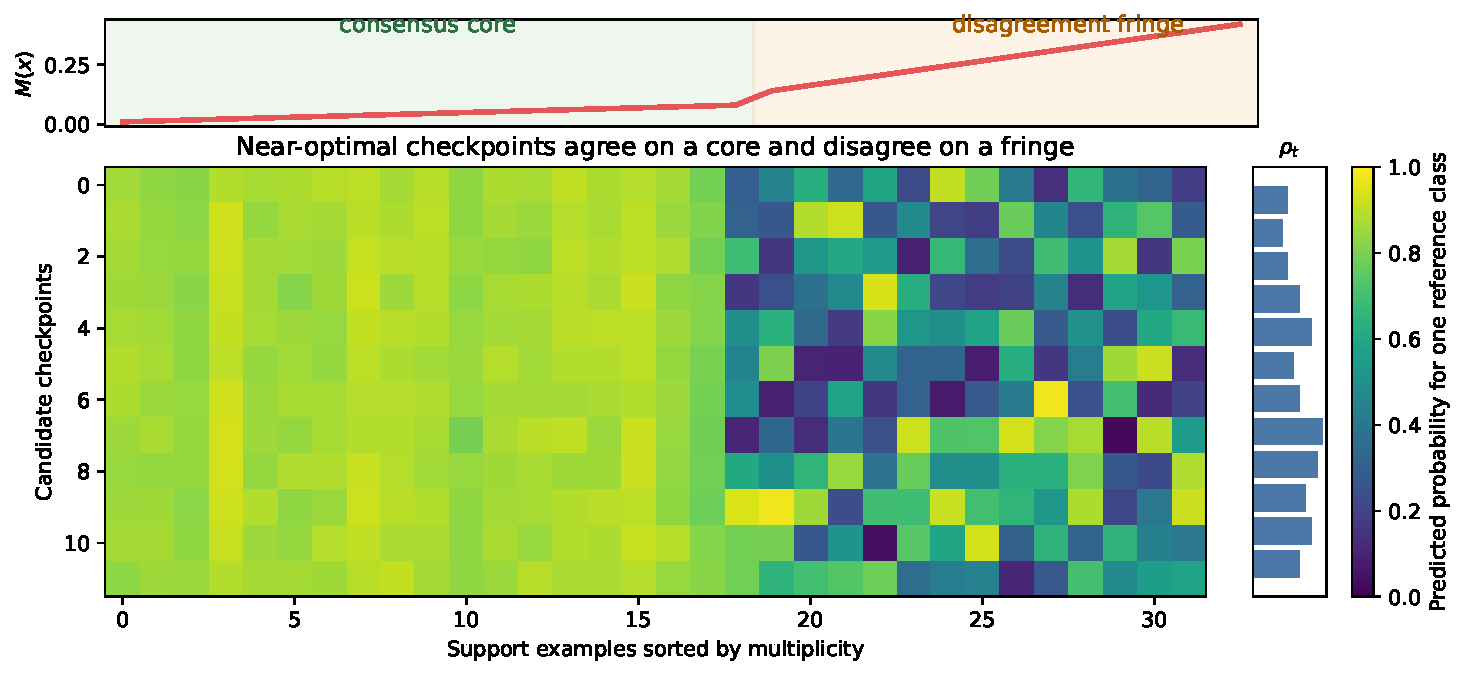
\includegraphics[width=\linewidth]{figures/consensus_core_heatmap.pdf}
    \caption{\textbf{Consensus core versus disagreement fringe.} Columns are support examples sorted by multiplicity; rows are candidate checkpoints. Vertically consistent columns form the consensus core, while striped columns form the high-multiplicity fringe. This is the object that \cora{} models directly and prior methods do not.}
    \label{fig:core}
\end{figure}

\begin{algorithm}[t]
    \caption{\cora{} (\textsc{Consensus-of-Rashomon Averaging})}
    \label{alg:cora}
    \begin{algorithmic}[1]
        \Require Dense checkpoints $\{\theta_t\}_{t=1}^{K}$, labeled validation set $\cV$, unlabeled support set $\cU$, tolerances $\epsilon,\tau$, and objective hyperparameters.
        \State Compute pooled validation losses $L_{\cV}(\theta_t)$ and choose anchor $a$ by Eq.~\eqref{eq:anchor}.
        \State Compute interpolation barriers $B(t,a)$ and form the connected near-optimal set $\cC$ by Eq.~\eqref{eq:candidate_set}.
        \State Compute trajectory prior $\rho_t$ on $\cC$ by Eq.~\eqref{eq:rho}.
        \For{each support example $x_i \in \cU$}
            \State Compute barycenter $q_i$ by Eq.~\eqref{eq:barycenter}.
            \State Compute multiplicity $M_i$ and core weight $c_i$ by Eqs.~\eqref{eq:multiplicity}--\eqref{eq:core_weight}.
        \EndFor
        \State Solve the convex simplex program in Eq.~\eqref{eq:optimizer}.
        \State Output the single weight soup $\bar\theta_{\cora}$ from Eq.~\eqref{eq:final_soup}.
    \end{algorithmic}
\end{algorithm}

\section{Theory}
\label{sec:theory}

\subsection{Convexity and optimization}

Throughout the theory section, we work with an $\eta$-clipped version of each predictive distribution,
\[
    \tilde p_t(x)
    \triangleq
    (1-K_{\mathrm{cls}}\eta)\,p_t(x) + \eta \mathbf{1},
    \qquad
    \eta \in (0,1/K_{\mathrm{cls}}],
\]
where $\mathbf{1}$ is the all-ones vector in $\RR^{K_{\mathrm{cls}}}$. This preserves the simplex constraint and guarantees every class probability lies in $[\eta,1]$. To keep notation light, we reuse $p_t$ for these clipped probabilities in the theorem statements below.

\begin{proposition}[Convexity, existence, and uniqueness]
\label{prop:convexity}
Under the clipping convention above, each term in Eq.~\eqref{eq:objective} is convex in $w$. Hence $J$ is convex on $\simplex^{|\cC|}$ and admits at least one minimizer. If $\lambda_{\mathrm{ent}} > 0$, the minimizer is unique.
\end{proposition}

\begin{proposition}[Projected-subgradient convergence for the non-entropic objective]
\label{prop:subgrad}
Assume $\lambda_{\mathrm{ent}} = 0$ and let $G$ be any Lipschitz constant of $J$ on $\simplex^{|\cC|}$ in $\ell_2$. Let $D$ be the Euclidean diameter of $\simplex^{|\cC|}$. Projected subgradient descent with step size
\[
    \eta_s = \frac{D}{G\sqrt{s}}
\]
returns averaged iterate $\bar w_S$ satisfying
\begin{equation}
    J(\bar w_S) - J(w^\star)
    \le
    \frac{DG}{\sqrt{S}}.
    \label{eq:subgrad_rate}
\end{equation}
\end{proposition}

\begin{remark}
If $\lambda_{\mathrm{ent}}>0$, the objective remains convex but is no longer globally Lipschitz on the closed simplex because of the boundary behavior of $w\log w$. In that case one can either optimize over a truncated simplex $w_t\ge \gamma$ or use entropic mirror descent. Our implementation uses a numerically stabilized simplex solver with a small positive floor.
\end{remark}

\subsection{A target-risk certificate from the consensus core}

The key theoretical move in \cora{} is to replace vague statements about flatness with an explicit decomposition of target uncertainty. Let $P_U$ denote the support-input distribution induced by the held-out support pool and let $P_T$ denote the unseen target input distribution. For each input $x$, define the population barycenter, multiplicity, and core weight by
\[
    q(x) \triangleq \sum_{t\in\cC}\rho_t p_t(x),
    \qquad
    M(x) \triangleq \sum_{t\in\cC}\rho_t \KL\!\big(p_t(x)\,\|\,q(x)\big),
    \qquad
    c(x) \triangleq \exp(-\kappa M(x)).
\]
For any feasible $w$, define the population support objective
\[
    \Omega(w)
    \triangleq
    \EE_{x\sim P_U}
    \Big[
        c(x)\KL\!\big(q(x)\,\|\,p_w(x)\big)
        +
        (1-c(x))A\!\big(p_w(x)\big)
    \Big].
\]
The empirical quantities $q_i$, $c_i$, and $\Omega_{\cU}(w)$ are the sample evaluations of these objects on the support sample $\cU$.

\begin{definition}[Consensus-fringe target decomposition]
\label{def:decomp}
Fix an input $x$. A target conditional label distribution $\pi_T(\cdot\mid x)$ admits a consensus-fringe decomposition with respect to $(q(x),c(x))$ if there exists some distribution $\nu_x$ such that
\begin{equation}
    \pi_T(\cdot\mid x)
    =
    c(x) q(x) + (1-c(x)) \nu_x,
    \qquad
    c(x)\in[0,1].
    \label{eq:decomp}
\end{equation}
\end{definition}

This assumption is stylized, but it is not circular. It says: on each input, the unseen target behaves partly like the trajectory consensus and partly like an arbitrary disagreement component. The job of \cora{} is to estimate which inputs are mostly one versus the other.

\begin{theorem}[Consensus-core certificate for predictive mixtures]
\label{thm:certificate}
Suppose the target conditional admits the decomposition in Definition~\ref{def:decomp} for measurable functions $q(x)$ and $c(x)$. Then for any predictive mixture $p_w$,
\begin{equation}
    \EE_{(x,y)\sim T}\big[-\log p_w(x)_y\big]
    \le
    C_T
    +
    \EE_{x\sim T}
    \Big[
        c(x)\KL\!\big(q(x)\,\|\,p_w(x)\big)
        +
        (1-c(x))A\!\big(p_w(x)\big)
    \Big],
    \label{eq:cert}
\end{equation}
where
\[
    C_T
    \triangleq
    \EE_{x\sim T}
    \Big[
        c(x)H\!\big(q(x)\big)
    \Big]
\]
is independent of $w$.
\end{theorem}

The theorem is the heart of the method. It says that if the target is well described by a consensus core plus an arbitrary fringe, then the right controllable terms are:
\begin{itemize}[leftmargin=1.4em]
    \item agreement with the consensus barycenter on core examples, and
    \item worst-case caution on the high-multiplicity fringe.
\end{itemize}
Those are exactly the support-side terms in Eq.~\eqref{eq:objective}.

\begin{remark}
The ambiguity term $A(p)=\max_y -\log p_y$ is not just a heuristic. Under log loss, it is the exact worst-case label risk at one input. This is why the paper uses it rather than a generic entropy regularizer as the primary theoretical object.
\end{remark}

\subsection{Empirical support estimation and concentration}

To connect Eq.~\eqref{eq:cert} to practice, we estimate the support-side terms from the held-out support pool $\cU$. Define
\begin{equation}
    \Omega_{\cU}(w)
    \triangleq
    \frac{1}{m}
    \sum_{i=1}^{m}
    \left[
        c_i \KL\!\big(q_i\,\|\,p_w(x_i)\big)
        +
        (1-c_i)A\!\big(p_w(x_i)\big)
    \right].
    \label{eq:omegaU}
\end{equation}

\begin{proposition}[Uniform concentration on the simplex]
\label{prop:concentration}
Under the clipping convention above, let $M = |\cC|$. For any $\varepsilon \in (0,1)$ and any $\delta\in(0,1)$, with probability at least $1-\delta$ over an \iid{} support sample of size $m$,
\begin{equation}
    \sup_{w\in\simplex^{M}}
    \left|
        \Omega_{\cU}(w) - \Omega(w)
    \right|
    \le
    \frac{4\varepsilon}{\eta}
    +
    \log\!\frac{1}{\eta}
    \sqrt{
        \frac{
            M\log(3/\varepsilon)+\log(2/\delta)
        }{
            2m
        }
    },
    \label{eq:uniform_conc}
\end{equation}
where $\Omega(w)$ is the corresponding population expectation under the support distribution.
\end{proposition}

For later use, define
\[
    \operatorname{Conc}(m,M,\delta,\eta,\varepsilon)
    \triangleq
    \frac{4\varepsilon}{\eta}
    +
    \log\!\frac{1}{\eta}
    \sqrt{
        \frac{
            M\log(3/\varepsilon)+\log(2/\delta)
        }{
            2m
        }
    }.
\]

\begin{corollary}[Density-ratio transfer]
\label{cor:density}
If the target input marginal is absolutely continuous with respect to the support distribution and satisfies
\[
    \frac{dP_T}{dP_U}(x) \le \rho
    \qquad
    \text{for all } x,
\]
then with the event of Proposition~\ref{prop:concentration},
\begin{equation}
    \EE_{x\sim T}
    \Big[
        c(x)\KL(q(x)\,\|\,p_w(x))
        +
        (1-c(x))A(p_w(x))
    \Big]
    \le
    \rho\,
    \Omega_{\cU}(w)
    +
    \rho\,
    \operatorname{Conc}(m,M,\delta,\eta,\varepsilon),
    \label{eq:density_transfer}
\end{equation}
uniformly over $w\in\simplex^M$.
\end{corollary}

\subsection{From predictive mixtures to a single weight soup}

The optimization in Eq.~\eqref{eq:objective} is over predictive mixtures. The final deployed object is a single soup $\bar\theta_w$. We therefore need a locality condition that transfers the certificate from the mixture to the actual weight average.

\begin{assumption}[Local second-order linearity]
\label{ass:locality}
For any feasible $w$, let
\[
    \bar\theta_w \triangleq \sum_{t\in\cC} w_t \theta_t.
\]
There exists $\Lambda > 0$ such that for every feasible $w$ and every support or validation input $x$,
\begin{equation}
    \norm{
        p_{\bar\theta_w}(x) - p_w(x)
    }_1
    \le
    \Lambda
    \sum_{t\in\cC}
    w_t
    \norm{\theta_t-\bar\theta_w}_2^2.
    \label{eq:locality_assump}
\end{equation}
\end{assumption}

\begin{theorem}[Mixture-to-soup discrepancy]
\label{thm:mixture_to_soup}
Under the clipping convention above and Assumption~\ref{ass:locality}, define the weighted trajectory variance
\[
    V(w)
    \triangleq
    \sum_{t\in\cC} w_t \norm{\theta_t-\bar\theta_w}_2^2.
\]
Then each of the three terms
\[
    L_{\cV}^{\mathrm{ens}}(w),
    \qquad
    \Omega_{\mathrm{core}}(w),
    \qquad
    \Omega_{\mathrm{amb}}(w)
\]
changes by at most $\Lambda \eta^{-1} V(w)$ when $p_w$ is replaced by the single soup $p_{\bar\theta_w}$. Consequently there exists a constant $C_{\mathrm{mix}}$ depending only on $\Lambda,\eta,\lambda_{\mathrm{core}},\lambda_{\mathrm{amb}}$ such that
\begin{equation}
    \big|J_{\mathrm{soup}}(w)-J(w)\big|
    \le
    C_{\mathrm{mix}} V(w),
    \label{eq:soup_gap}
\end{equation}
where $J_{\mathrm{soup}}$ denotes the same objective evaluated at the deployed soup predictions.
\end{theorem}

\subsection{How \cora{} compares to \swad}

The strongest honest theorem is a conditional domination result. \swad{} selects a contiguous interval and averages uniformly. If such an interval lies inside $\cC$, its uniform weights define a feasible point of the \cora{} simplex.

\begin{definition}[Feasible \swad-style interval]
Let $\cI$ be the set of contiguous intervals $I\subseteq\cC$. For each $I\in\cI$, define its uniform weight vector $u_I$ by
\[
    (u_I)_t
    =
    \begin{cases}
        |I|^{-1}, & t\in I,\\
        0, & t\notin I.
    \end{cases}
\]
\end{definition}

\begin{corollary}[Optimization consequence relative to feasible \swad-style intervals]
\label{thm:domination}
Suppose there exist constants $\Gamma,\alpha,\beta \ge 0$ such that for every feasible $w\in\simplex^{|\cC|}$,
\begin{equation}
    R_T^{\mathrm{ens}}(w)
    \le
    \Gamma
    +
    \alpha J(w)
    +
    \beta V(w),
    \label{eq:dom_assump}
\end{equation}
where $R_T^{\mathrm{ens}}(w)$ is the target log loss of the predictive mixture and $V(w)$ is defined above. Let $w^\star$ minimize $J$. Then for every feasible \swad-style interval $I\in\cI$,
\begin{equation}
    R_T^{\mathrm{ens}}(w^\star)
    \le
    \Gamma
    +
    \alpha J(u_I)
    +
    \beta V(w^\star).
    \label{eq:domination}
\end{equation}
If, in addition, $V(w^\star)\le V(u_I)$ for the interval under comparison, then the \cora{} certificate is no worse than the certificate of that interval.
\end{corollary}

This is the correct comparison to \swad{}. It does not claim that \cora{} always wins empirically. It claims that once the target-risk certificate is accepted, \cora{} is optimizing over a strictly richer feasible family than uniform contiguous intervals.

\subsection{Constructive separation}

\begin{proposition}[Constructive separation from validation-only selection]
\label{thm:separation}
For every clipping level $\eta \in (0,\nicefrac{1}{2})$, there exists a binary classification problem with one core example $x_c$, one fringe example $x_f$, and two feasible post-hoc soups $w_A,w_B$ such that:
\begin{enumerate}[leftmargin=1.4em]
    \item $w_A$ and $w_B$ have the same validation loss on $\cV$;
    \item any selector that depends only on pooled validation loss is indifferent between them;
    \item \cora{} strictly prefers $w_B$;
    \item the worst-case single-input target log loss of $w_B$ is strictly lower than that of $w_A$ by at least $\log(1/\eta)-\log 2$.
\end{enumerate}
\end{proposition}

The construction is simple. Both soups agree perfectly on the validation example $x_c$. On $x_f$, soup $w_A$ predicts $(1-\eta,\eta)$ while soup $w_B$ predicts $(\nicefrac{1}{2},\nicefrac{1}{2})$. Since $x_f$ lies entirely in the disagreement fringe, \cora{} uses the ambiguity term and prefers $w_B$. If the target label at $x_f$ is arbitrary or unknown, the worst-case log loss of $w_A$ is $\log(1/\eta)$ while that of $w_B$ is $\log 2$. Flatness-only or drift-only selectors can still miss this distinction whenever their external summaries tie, but the theorem itself only needs the validation-equivalence claim.

\begin{figure}[t]
    \centering
    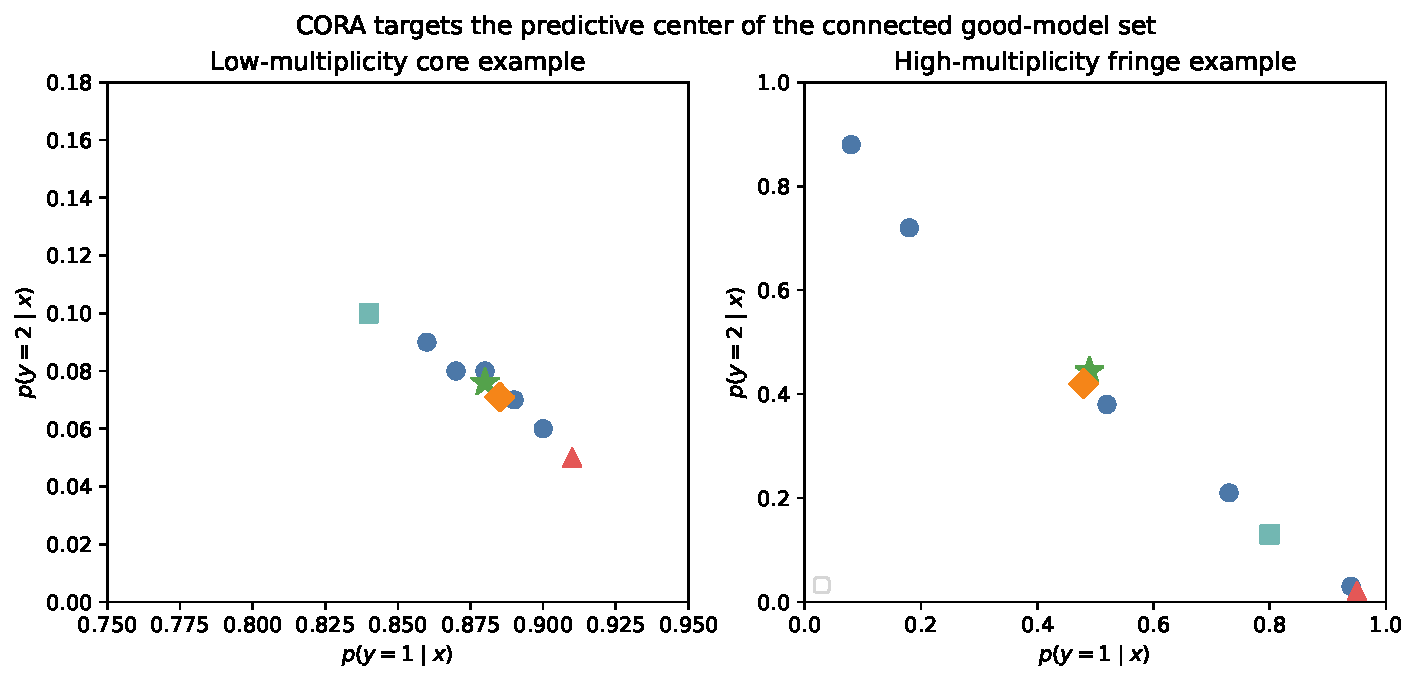
\includegraphics[width=\linewidth]{figures/barycenter_geometry.pdf}
    \caption{\textbf{Prediction-space geometry.} For a fixed example, candidate checkpoint predictions can disagree substantially while remaining equally low-loss globally. \cora{} targets the barycenter on low-multiplicity examples and avoids brittle fringe commitments.}
    \label{fig:geometry}
\end{figure}

\begin{figure}[t]
    \centering
    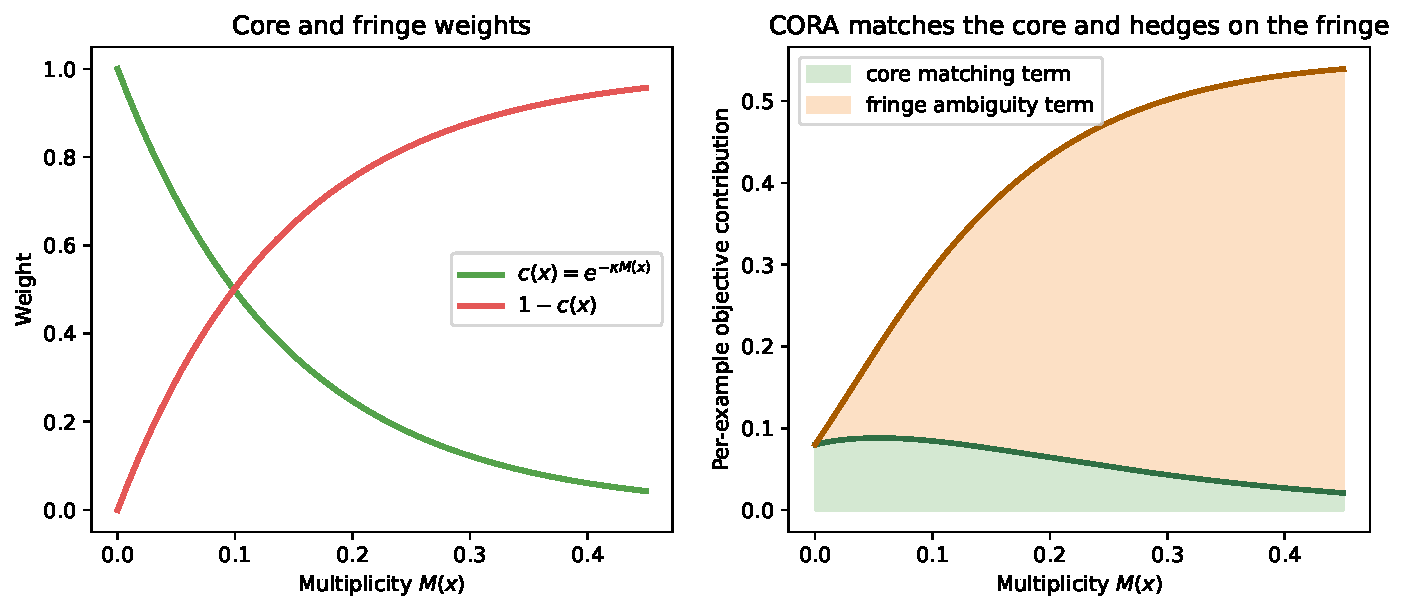
\includegraphics[width=\linewidth]{figures/objective_decomposition.pdf}
    \caption{\textbf{Core matching versus fringe hedging.} The \cora{} objective emphasizes barycenter matching where multiplicity is low and worst-case caution where multiplicity is high. This differs structurally from both flatness-only and drift-only selectors.}
    \label{fig:objective}
\end{figure}

\section{Empirical Protocol}
\label{sec:experiments}

All new \cora{} results are intentionally left as \TBD{}. This section records the protocol required to test the method cleanly against the current frontier.

\paragraph{Datasets and protocol.}
We will follow the standard DomainBed protocol on PACS, VLCS, OfficeHome, TerraIncognita, and DomainNet \citep{gulrajani2021domainbed,cha2021swad}. We will report average out-of-domain accuracy over target domains and three seeds, together with datasetwise breakdowns and confidence intervals where appropriate.

\paragraph{Base training.}
\cora{} is post-hoc and single-run. Each experiment therefore consists of:
\begin{itemize}[leftmargin=1.4em]
    \item ordinary base training,
    \item dense checkpoint saving,
    \item one post-hoc selection/souping pass,
    \item one test-time model.
\end{itemize}

\paragraph{Decisive analyses.}
The most important analyses are not only top-line benchmark averages.
\begin{enumerate}[leftmargin=1.4em]
    \item Correlation between per-example multiplicity $M_i$ and held-out target error.
    \item Matched-checkpoint-set comparisons where loss and barrier are similar but multiplicity structure differs.
    \item Ablations removing the core term, ambiguity term, locality gate, and prior $\rho_t$.
    \item Replay comparisons on the exact same dense checkpoint trajectory against `ERM`, `\swad`, `\stawa`, and `\dcola`.
\end{enumerate}

\subsection{Published baseline numbers}

Table~\ref{tab:published} records exact numbers from published work that define the current benchmark landscape. They are included for context only. They are not a substitute for running \cora{}.

\begin{table}[t]
    \centering
    \small
    \caption{\textbf{Published five-dataset ResNet-50-style benchmark numbers from prior work.} Numbers come from the cited source tables and are not from identical protocols; in particular, \diwa{} is primarily multi-run and \miro{} is training-time rather than post-hoc.}
    \label{tab:published}
    \begin{adjustbox}{width=\textwidth}
    \begin{tabular}{lcccccc}
        \toprule
        Method & PACS & VLCS & OfficeHome & TerraInc. & DomainNet & Avg. \\
        \midrule
        ERM \citep{cha2021swad} & 85.5 & 77.5 & 66.5 & 46.1 & 40.9 & 63.3 \\
        ERM + SWA$_{\mathrm{const}}$ \citep{cha2021swad} & 86.9 & 76.6 & 69.3 & 49.2 & 45.9 & 65.6 \\
        ERM + \swad{} \citep{cha2021swad} & 88.1 & 79.1 & 70.6 & 50.0 & 46.5 & 66.9 \\
        MA \citep{rame2022diwa} & 87.5 & 78.2 & 70.6 & 50.3 & 46.0 & 66.5 \\
        \diwa{}$^\dagger$ \citep{rame2022diwa} & 89.0 & 78.6 & 72.8 & 51.9 & 47.7 & 68.0 \\
        \miro{} \citep{cha2022miro} & 85.4 & 79.0 & 70.5 & 50.4 & 44.3 & 65.9 \\
        \miro{} + \swad{} \citep{cha2022miro} & 88.4 & 79.6 & 72.4 & 52.9 & 47.0 & 68.1 \\
        \bottomrule
    \end{tabular}
    \end{adjustbox}
\end{table}

\subsection{Planned \cora{} tables}

\begin{table}[t]
    \centering
    \small
    \caption{\textbf{Planned \cora{} benchmark results.} All entries remain intentionally blank pending experiments.}
    \label{tab:tbd}
    \begin{tabular}{lcccccc}
        \toprule
        Method & PACS & VLCS & OfficeHome & TerraInc. & DomainNet & Avg. \\
        \midrule
        ERM replay & \TBD{} & \TBD{} & \TBD{} & \TBD{} & \TBD{} & \TBD{} \\
        \swad{} replay & \TBD{} & \TBD{} & \TBD{} & \TBD{} & \TBD{} & \TBD{} \\
        \stawa{} replay & \TBD{} & \TBD{} & \TBD{} & \TBD{} & \TBD{} & \TBD{} \\
        \dcola{} replay & \TBD{} & \TBD{} & \TBD{} & \TBD{} & \TBD{} & \TBD{} \\
        \cora{} & \TBD{} & \TBD{} & \TBD{} & \TBD{} & \TBD{} & \TBD{} \\
        \bottomrule
    \end{tabular}
\end{table}

\section{Discussion}

\paragraph{Why \cora{} is not a disguised window selector.}
The main scientific failure mode of many post-hoc ideas is reduction to “better timing.” \cora{} is designed to resist that attack. Its core object, the examplewise multiplicity structure of the connected candidate set, cannot be reduced to one scalar trace over time. If two candidate checkpoint collections have comparable validation loss and barrier profiles but different consensus-core structure, \cora{} can rank them differently by construction.

\paragraph{Why the method is still simple enough to spread.}
Even though the theory is richer than \swad{}'s slogan, the operational recipe is still short:
\begin{enumerate}[leftmargin=1.4em]
    \item find the connected near-optimal checkpoints,
    \item compute the predictive barycenter and multiplicity,
    \item solve one convex simplex problem,
    \item output one soup.
\end{enumerate}
That is meaningfully simpler than training-time DG objectives or multi-run ensembles.

\paragraph{Limitations.}
The paper has several honest limitations.
\begin{itemize}[leftmargin=1.4em]
    \item The strongest target-risk theorem uses an explicit consensus-fringe decomposition. This is a real modeling assumption, not a universal truth.
    \item The deployed model is a weight soup, so the predictive-mixture certificate still requires a locality approximation to transfer cleanly.
    \item The current manuscript includes no new \cora{} benchmark results yet. It is structurally ready for publication, but not empirically submission-ready until the \TBD{} sections are replaced.
    \item The theory is developed for multiclass classification. The same principle should transfer to other proper-loss settings, but that extension is not fully derived here.
    \item The method may collapse toward plain soups if multiplicity structure turns out not to be informative on a given trajectory. This is an empirical question and must be tested directly.
\end{itemize}

\section{Conclusion}

\cora{} proposes a different answer to the single-run post-hoc DG problem. The key object is not a flat late basin, not a calm late checkpoint, and not checkpoint-level diversity alone. It is the predictive consensus core of the connected good-model set. The resulting method keeps the deployment simplicity that made \swad{} influential while opening a different theory route: target robustness can be controlled by barycenter matching on low-multiplicity examples and worst-case caution on the high-multiplicity fringe. Whether that object is strong enough to beat the field consistently remains an empirical question. This manuscript makes that question precise.

\newpage
\appendix

\section{Proofs}

\subsection{Proof of Theorem~\ref{thm:barycenter}}

\begin{proof}
Fix $x_i$ and abbreviate $p_t = p_t(x_i)$. Consider
\[
    F(r)
    =
    \sum_{t\in\cC}\rho_t \KL(p_t \,\|\, r)
    =
    \sum_{t\in\cC}\rho_t
    \sum_{y=1}^{K_{\mathrm{cls}}}
    p_{t,y}\log\frac{p_{t,y}}{r_y}.
\]
The terms involving $\log p_{t,y}$ are constant in $r$, so minimizing $F$ is equivalent to minimizing
\[
    G(r)
    =
    - \sum_{y=1}^{K_{\mathrm{cls}}}
    \left(
        \sum_{t\in\cC}\rho_t p_{t,y}
    \right)
    \log r_y
    =
    -\sum_{y=1}^{K_{\mathrm{cls}}} q_{i,y}\log r_y
    .
\]
This is the cross-entropy from $q_i$ to $r$. Over the closed simplex, by Gibbs' inequality,
\[
    G(r) - G(q_i)
    =
    \KL(q_i \,\|\, r)
    \ge 0
    .
\]
Hence $q_i$ minimizes $G$, and therefore $F$. If $q_{i,y}>0$ for every class $y$, then $\KL(q_i\|r)=0$ implies $r=q_i$, so the minimizer is unique.
\end{proof}

\subsection{Proof of Proposition~\ref{prop:convexity}}

\begin{proof}
Each term is convex in $w$:
\begin{enumerate}[leftmargin=1.4em]
    \item In Eq.~\eqref{eq:ensval}, each summand is
    \[
        -\log\!\left(\sum_{t\in\cC} w_t p_t(x_j)_{y_j}\right),
    \]
    a composition of the convex decreasing map $-\log$ with an affine positive function of $w$.
    \item In Eq.~\eqref{eq:core_term}, the terms
    \[
        \KL(q_i\|p_w(x_i))
        =
        \sum_y q_{i,y}\log \frac{q_{i,y}}{(p_w(x_i))_y}
    \]
    are also convex for the same reason.
    \item In Eq.~\eqref{eq:amb_term}, $A(p_w(x_i))$ is the maximum of the convex functions
    \[
        -\log (p_w(x_i))_y,
    \]
    so it is convex.
    \item The locality term is linear.
    \item The entropy term $\sum_t w_t\log w_t$ is strictly convex on the simplex interior.
\end{enumerate}
Therefore $J$ is convex. Since the simplex is compact and $J$ is continuous under the clipping convention above, a minimizer exists. If $\lambda_{\mathrm{ent}}>0$, strict convexity of the entropy term makes $J$ strictly convex, hence the minimizer is unique.
\end{proof}

\subsection{Proof of Proposition~\ref{prop:subgrad}}

\begin{proof}
Under the clipping convention and $\lambda_{\mathrm{ent}}=0$, every probability appearing inside a logarithm is at least $\eta$, so the subgradients contributed by the validation, core, ambiguity, and locality terms are bounded uniformly on the compact simplex. Thus $J$ is $G$-Lipschitz on the simplex. The claimed rate is the standard projected-subgradient guarantee for convex $G$-Lipschitz objectives over a set of diameter $D$:
\[
    J(\bar w_S)-J(w^\star)
    \le
    \frac{D^2 + G^2\sum_{s=1}^{S}\eta_s^2}{2\sum_{s=1}^{S}\eta_s}
    \le
    \frac{DG}{\sqrt{S}}.
\]
The final inequality follows by substituting $\eta_s = D/(G\sqrt{s})$ and using the usual harmonic-square-root bounds.
\end{proof}

\subsection{Proof of Theorem~\ref{thm:certificate}}

\begin{proof}
Fix $x$ and write $\pi = \pi_T(\cdot\mid x)$, $q=q(x)$, $c=c(x)$, and $\nu=\nu_x$. By Definition~\ref{def:decomp},
\[
    \pi = c q + (1-c)\nu.
\]
For any predictive distribution $p$,
\begin{align*}
    \EE_{y\sim\pi}\big[-\log p_y\big]
    &=
    c\, \EE_{y\sim q}\big[-\log p_y\big]
    +
    (1-c)\, \EE_{y\sim \nu}\big[-\log p_y\big] \\
    &=
    c\Big(H(q)+\KL(q\|p)\Big)
    +
    (1-c)\, \EE_{y\sim\nu}\big[-\log p_y\big].
\end{align*}
For the fringe term,
\[
    \EE_{y\sim\nu}\big[-\log p_y\big]
    \le
    \max_y -\log p_y
    =
    A(p).
\]
Hence
\[
    \EE_{y\sim\pi}\big[-\log p_y\big]
    \le
    cH(q)
    +
    c\KL(q\|p)
    +
    (1-c)A(p).
\]
Integrating over $x\sim T$ yields Eq.~\eqref{eq:cert}, with the constant term collecting the entropy of the consensus component:
\[
    C_T
    =
    \EE_{x\sim T}\big[c(x)H(q(x))\big].
\]
\end{proof}

\subsection{Proof of Proposition~\ref{prop:concentration}}

\begin{proof}
Under the clipping convention above,
\[
    0 \le \KL(q_i\|p_w(x_i)) \le \log(1/\eta),
    \qquad
    0 \le A(p_w(x_i)) \le \log(1/\eta).
\]
Therefore each summand of $\Omega_{\cU}(w)$ is bounded in $[0,\log(1/\eta)]$.

Next, for any two weights $w,w'$, each coordinate of $p_w(x_i)$ is affine in $w$, and on the $\eta$-clipped simplex the map $u\mapsto -\log u$ is $1/\eta$-Lipschitz. Hence
\[
    \left|
        \Omega_{\cU}(w)-\Omega_{\cU}(w')
    \right|
    \le
    \frac{2}{\eta}\norm{w-w'}_1.
\]
Let $\mathcal N_{\varepsilon}$ be an $\varepsilon$-net of $\simplex^M$ in $\ell_1$ with cardinality at most $(3/\varepsilon)^M$. For each $u\in\mathcal N_{\varepsilon}$, Hoeffding's inequality gives
\[
    \Pr\Big(
        |\Omega_{\cU}(u)-\Omega(u)| > t
    \Big)
    \le
    2\exp\!\left(
        -\frac{2m t^2}{\log^2(1/\eta)}
    \right).
\]
Union bound over the net gives that with probability at least $1-\delta$,
\[
    \max_{u\in\mathcal N_{\varepsilon}}
    |\Omega_{\cU}(u)-\Omega(u)|
    \le
    \log\!\frac{1}{\eta}
    \sqrt{
        \frac{M\log(3/\varepsilon)+\log(2/\delta)}{2m}
    }.
\]
Finally, for arbitrary $w$, choose $u\in\mathcal N_\varepsilon$ with $\norm{w-u}_1\le\varepsilon$ and use the Lipschitz bound on both empirical and population terms:
\[
    |\Omega_{\cU}(w)-\Omega(w)|
    \le
    |\Omega_{\cU}(u)-\Omega(u)|
    +
    \frac{4\varepsilon}{\eta}.
\]
This yields Eq.~\eqref{eq:uniform_conc}.
\end{proof}

\subsection{Proof of Corollary~\ref{cor:density}}

\begin{proof}
Let
\[
    \phi_w(x)
    =
    c(x)\KL(q(x)\|p_w(x))
    +
    (1-c(x))A(p_w(x)).
\]
Then
\[
    \EE_{x\sim T}[\phi_w(x)]
    =
    \EE_{x\sim U}\!\left[\frac{dP_T}{dP_U}(x)\phi_w(x)\right]
    \le
    \rho\, \EE_{x\sim U}[\phi_w(x)]
    =
    \rho\, \Omega(w).
\]
Apply Proposition~\ref{prop:concentration} to replace $\Omega(w)$ with $\Omega_{\cU}(w)$ plus the concentration term.
\end{proof}

\subsection{Proof of Theorem~\ref{thm:mixture_to_soup}}

\begin{proof}
Fix any support or validation input $x$. By Assumption~\ref{ass:locality},
\[
    \norm{p_{\bar\theta_w}(x)-p_w(x)}_1
    \le
    \Lambda V(w).
\]
For any class $y$, the map $p\mapsto -\log p_y$ is $1/\eta$-Lipschitz on the $\eta$-clipped simplex, so
\[
    \left|
        -\log p_{\bar\theta_w}(x)_y
        +
        \log p_w(x)_y
    \right|
    \le
    \frac{\Lambda}{\eta}V(w).
\]
Since $A(p)=\max_y -\log p_y$ is the maximum of $1/\eta$-Lipschitz functions, it is also $1/\eta$-Lipschitz in $\ell_1$. The same bound applies to $\KL(q\|p)$ because
\[
    \left|
        \KL(q\|p)-\KL(q\|p')
    \right|
    =
    \left|
        \sum_y q_y \log \frac{p'_y}{p_y}
    \right|
    \le
    \frac{1}{\eta}\norm{p-p'}_1.
\]
Averaging over support or validation samples yields the same $\Lambda\eta^{-1}V(w)$ bound for each certificate term. Summing them with coefficients gives Eq.~\eqref{eq:soup_gap}.
\end{proof}

\subsection{Proof of Corollary~\ref{thm:domination}}

\begin{proof}
Because each feasible interval weight vector $u_I$ lies in the simplex over $\cC$,
\[
    J(w^\star) \le J(u_I)
    \qquad
    \text{for every } I\in\cI.
\]
Combining this with the assumed certificate Eq.~\eqref{eq:dom_assump} yields
\[
    R_T^{\mathrm{ens}}(w^\star)
    \le
    \Gamma + \alpha J(w^\star) + \beta V(w^\star)
    \le
    \Gamma + \alpha J(u_I) + \beta V(w^\star).
\]
This is exactly Eq.~\eqref{eq:domination}. If $V(w^\star)\le V(u_I)$, the right-hand side is no larger than the corresponding certificate for the interval.
\end{proof}

\subsection{Proof of Proposition~\ref{thm:separation}}

\begin{proof}
Take binary classification with two support examples $x_c,x_f$. Let the validation set contain only $(x_c,1)$. Let two candidate soups produce the following predictions:
\[
    p_A(x_c)=p_B(x_c)=(1-\eta,\eta),
\]
and on the fringe point
\[
    p_A(x_f)=(1-\eta,\eta),
    \qquad
    p_B(x_f)=\left(\tfrac12,\tfrac12\right).
\]
By construction, both soups have the same validation loss because they agree on $x_c$ and the validation set ignores $x_f$.
Now let the target decomposition satisfy
\[
    c(x_c)=1,
    \qquad
    c(x_f)=0.
\]
Then the \cora{} support-side preference on the fringe is entirely through the ambiguity term:
\[
    A(p_A(x_f)) = \log(1/\eta),
    \qquad
    A(p_B(x_f)) = \log 2.
\]
Since $\eta < \nicefrac12$, we have $\log(1/\eta) > \log 2$, so \cora{} strictly prefers $w_B$.

Finally, if the target label at $x_f$ is arbitrary, the worst-case log loss of $p_A$ at $x_f$ is $\log(1/\eta)$, while the worst-case log loss of $p_B$ is $\log 2$. Therefore the target-risk gap is at least $\log(1/\eta)-\log 2 > 0$.
\end{proof}

\section{Additional Baseline Notes}

\paragraph{\swad{} versus \diwa{} versus \miro{}.}
The published numbers in Table~\ref{tab:published} mix related but not identical regimes:
\begin{itemize}[leftmargin=1.4em]
    \item \swad{} is the cleanest single-run post-hoc baseline.
    \item \diwa{} is mostly a multi-run diversity method.
    \item \miro{} is training-time regularization, while \miro{} + \swad{} is a training-time plus post-hoc combination.
\end{itemize}
This is why the fairest immediate comparison for \cora{} is against single-run replayed `ERM`, `\swad`, `\stawa`, and `\dcola` on identical checkpoint trajectories.

\section{Additional Visual Comparison}

\begin{figure}[h]
    \centering
    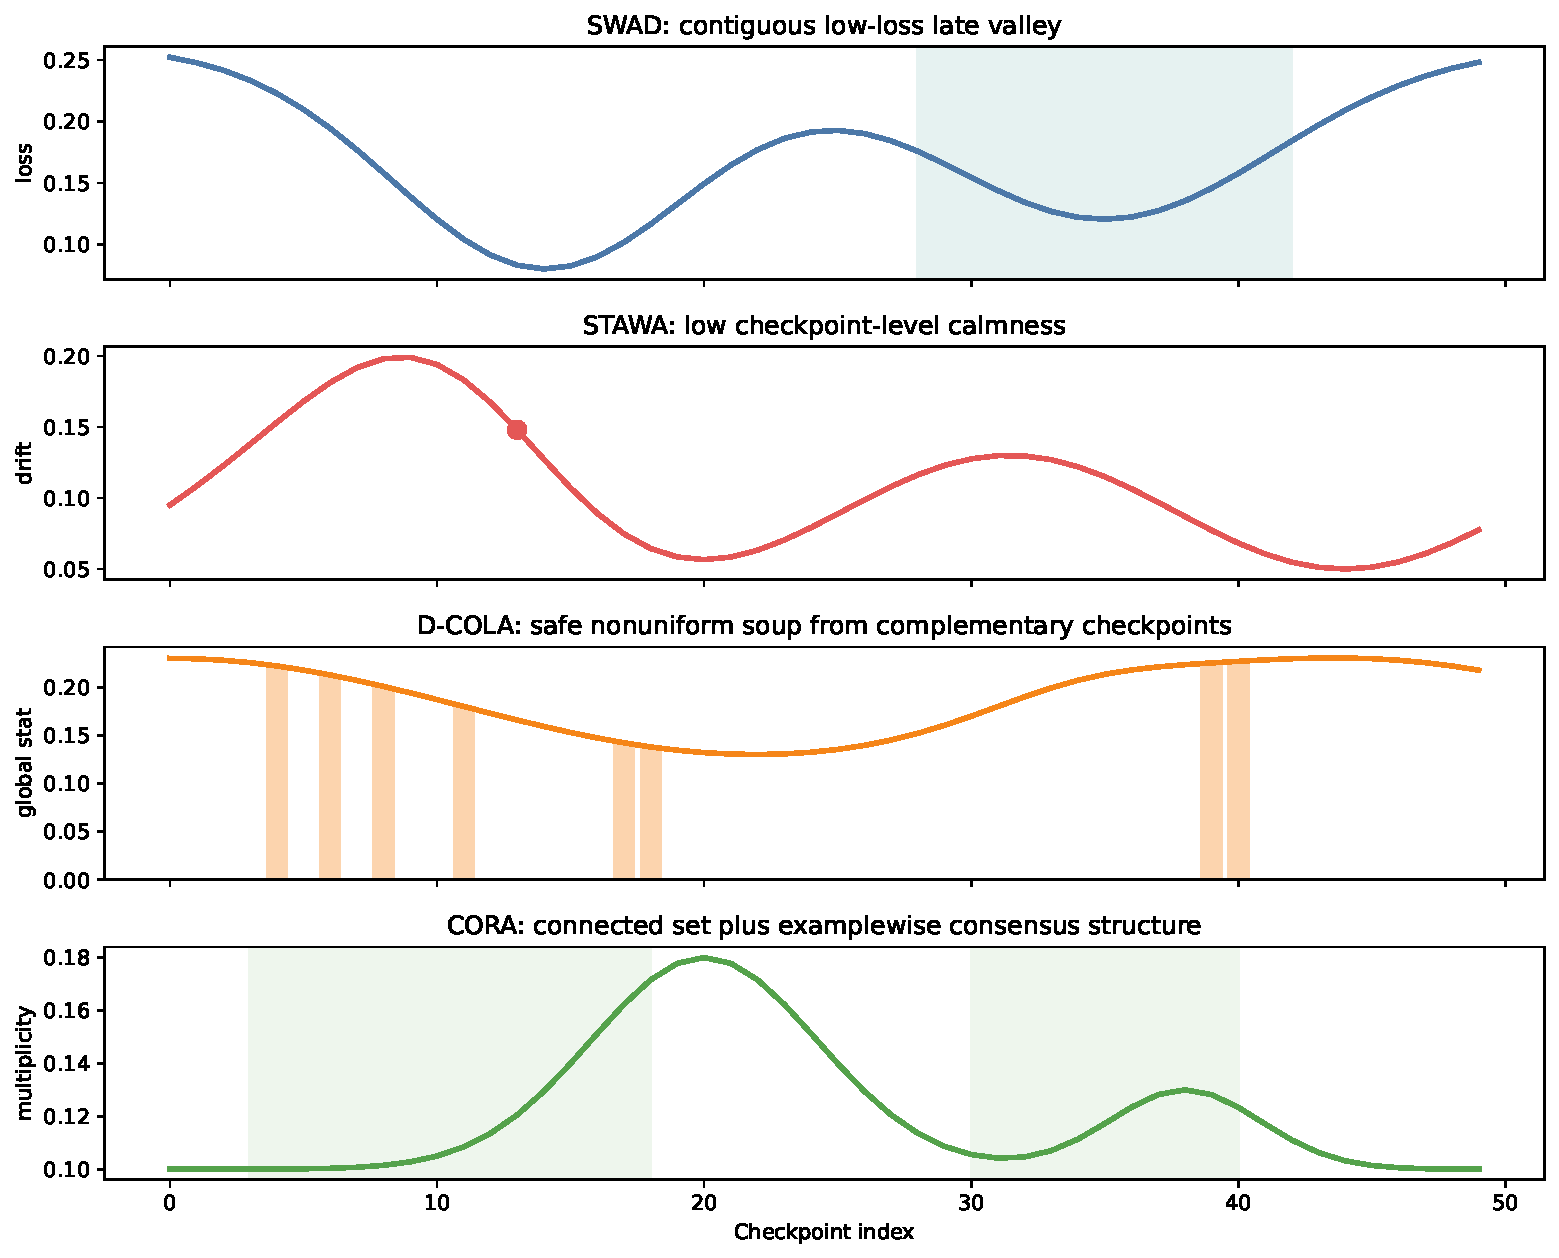
\includegraphics[width=\linewidth]{figures/method_contrast.pdf}
    \caption{\textbf{Conceptual contrast among post-hoc selectors.} \swad{} emphasizes connected flat valleys, stationarity-style methods emphasize temporal calmness, and \cora{} emphasizes examplewise consensus inside the connected good-model set.}
\end{figure}

\bibliographystyle{plainnat}
\bibliography{references}

\end{document}
